\documentclass[tikz]{standalone}

\usepackage{tikz}
\usetikzlibrary{shapes}
\usetikzlibrary{decorations.pathreplacing}
\usetikzlibrary{hobby,backgrounds,calc,trees}
\colorlet{lgray}{gray!25}
\colorlet{llgray}{gray!50}

\newcommand{\convexpath}[2]{
[   
    create hullnodes/.code={
        \global\edef\namelist{#1}
        \foreach [count=\counter] \nodename in \namelist {
            \global\edef\numberofnodes{\counter}
            \node at (\nodename) [draw=none,name=hullnode\counter] {};
        }
        \node at (hullnode\numberofnodes) [name=hullnode0,draw=none] {};
        \pgfmathtruncatemacro\lastnumber{\numberofnodes+1}
        \node at (hullnode1) [name=hullnode\lastnumber,draw=none] {};
    },
    create hullnodes
]
($(hullnode1)!#2!-90:(hullnode0)$)
\foreach [
    evaluate=\currentnode as \previousnode using \currentnode-1,
    evaluate=\currentnode as \nextnode using \currentnode+1
    ] \currentnode in {1,...,\numberofnodes} {
  let
    \p1 = ($(hullnode\currentnode)!#2!-90:(hullnode\previousnode)$),
    \p2 = ($(hullnode\currentnode)!#2!90:(hullnode\nextnode)$),
    \p3 = ($(\p1) - (hullnode\currentnode)$),
    \n1 = {atan2(\y3,\x3)},
    \p4 = ($(\p2) - (hullnode\currentnode)$),
    \n2 = {atan2(\y4,\x4)},
    \n{delta} = {-Mod(\n1-\n2,360)}
  in 
    {-- (\p1) arc[start angle=\n1, delta angle=\n{delta}, radius=#2] -- (\p2)}
}
-- cycle
}

\begin{document}
%
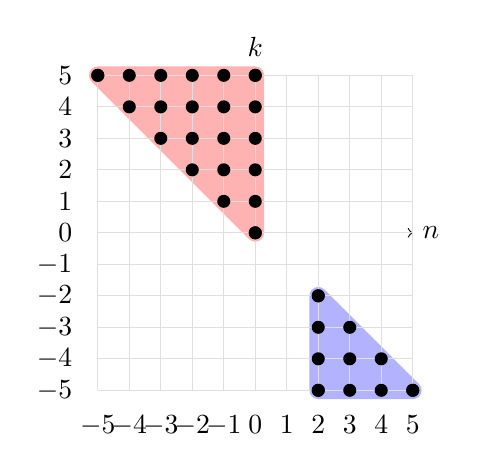
\begin{tikzpicture}[scale=0.4]
\draw[->] (-5,0)--(5,0);
\draw[->] (0,-5)--(0,5);
\draw[help lines, thin, lgray] (-5,-5) grid (5,5);
\node[right] at (5,0) {$n$};
\foreach \x in {-5,...,5}{
   \node[left] at (-5.5,\x) {$\x$}; 
}
\foreach \x in {-5,...,5}{
   \node[below] at (\x,-5.5) {$\x$}; 
}
\node[above] at (0,5.3) {$k$};
\foreach \x in {2,3,4,5}{
    \foreach \y in {-2,-3,-4,-5}{
        \ifnum\x<\numexpr-\y+1
            \node[circle,fill,scale=0.5] at (\x,\y){};
        \fi
    }
}
\foreach \x in {0,...,-5}{
    \foreach \y in {0,...,5}{
        \ifnum\x>\numexpr-\y-1
            \node[circle,fill,scale=0.5] at (\x,\y){};
        \fi
    }
}
\node[circle,fill,scale=0.5] (a) at (2,-2){};
\node[circle,fill,scale=0.5] (b) at (2,-5){};
\node[circle,fill,scale=0.5] (c) at (5,-5){};
\node[circle,fill,scale=0.5] (d) at (0,0){};
\node[circle,fill,scale=0.5] (e) at (-5,5){};
\node[circle,fill,scale=0.5] (f) at (0,5){};
\begin{pgfonlayer}{background}
    % the requested case
\fill[blue,opacity=0.3] \convexpath{a,c,b}{8pt};
\fill[red,opacity=0.3] \convexpath{d,e,f}{8pt};
\end{pgfonlayer}
\end{tikzpicture}
%
\end{document}